\documentclass[./]{subfiles}

%Bezier Extraction
\begin{document}
B\`{e}zier extraction, discussed at length in \cite{borden_isogeometric_2011} fundamentally links the the B-spline basis technology of IGA with the data structures prevalent in classical Finite Elements. As illustrated above, B-spline bases have support spanning several elements (knot spans). This extended support is partially responsible for the improved accuracy of IGA over typical Finite element methods, though it is also fundamentally incompatible with current discretization technologies widely employed for performing Finite Element Analysis. Specifically, classical Finite elements relies on a straightforward pull back from an element in the parametric domain to a parent element. This mapping is simple because typical bases utilized in classical Finite Elements are designed strictly with local support over an element in parametric space. The concept of a parent element is important to the implementation of classical Finite Elements, as information about basis functions and quadrature must only be stored for a single element, as opposed to having bases evaluated at quadrature points over every element in the domain. The parent element dramatically reduces the memory cost of Finite Elements and is thus ubiquitous in Finite Element packages. This presents a problem for our B-spline bases, as they do not have local support, we must store basis information over each element. Fortunately, through the extraction operator, we may convert our B-spline bases to Bernstein bases with local support over each element (knot span). This mapping is performed through the \textit{extraction operator}. 

The extraction operator maps Bernstein polynomials to B-spline bases via a simple linear combination.  As such, a single Bernstein parent element can be employed to integrate B-spline bases into a typical Finite Element data structure. These two sets of bases are shown side by side in Figure \ref{fig:extracted}. 

\begin{figure}
  \centerline{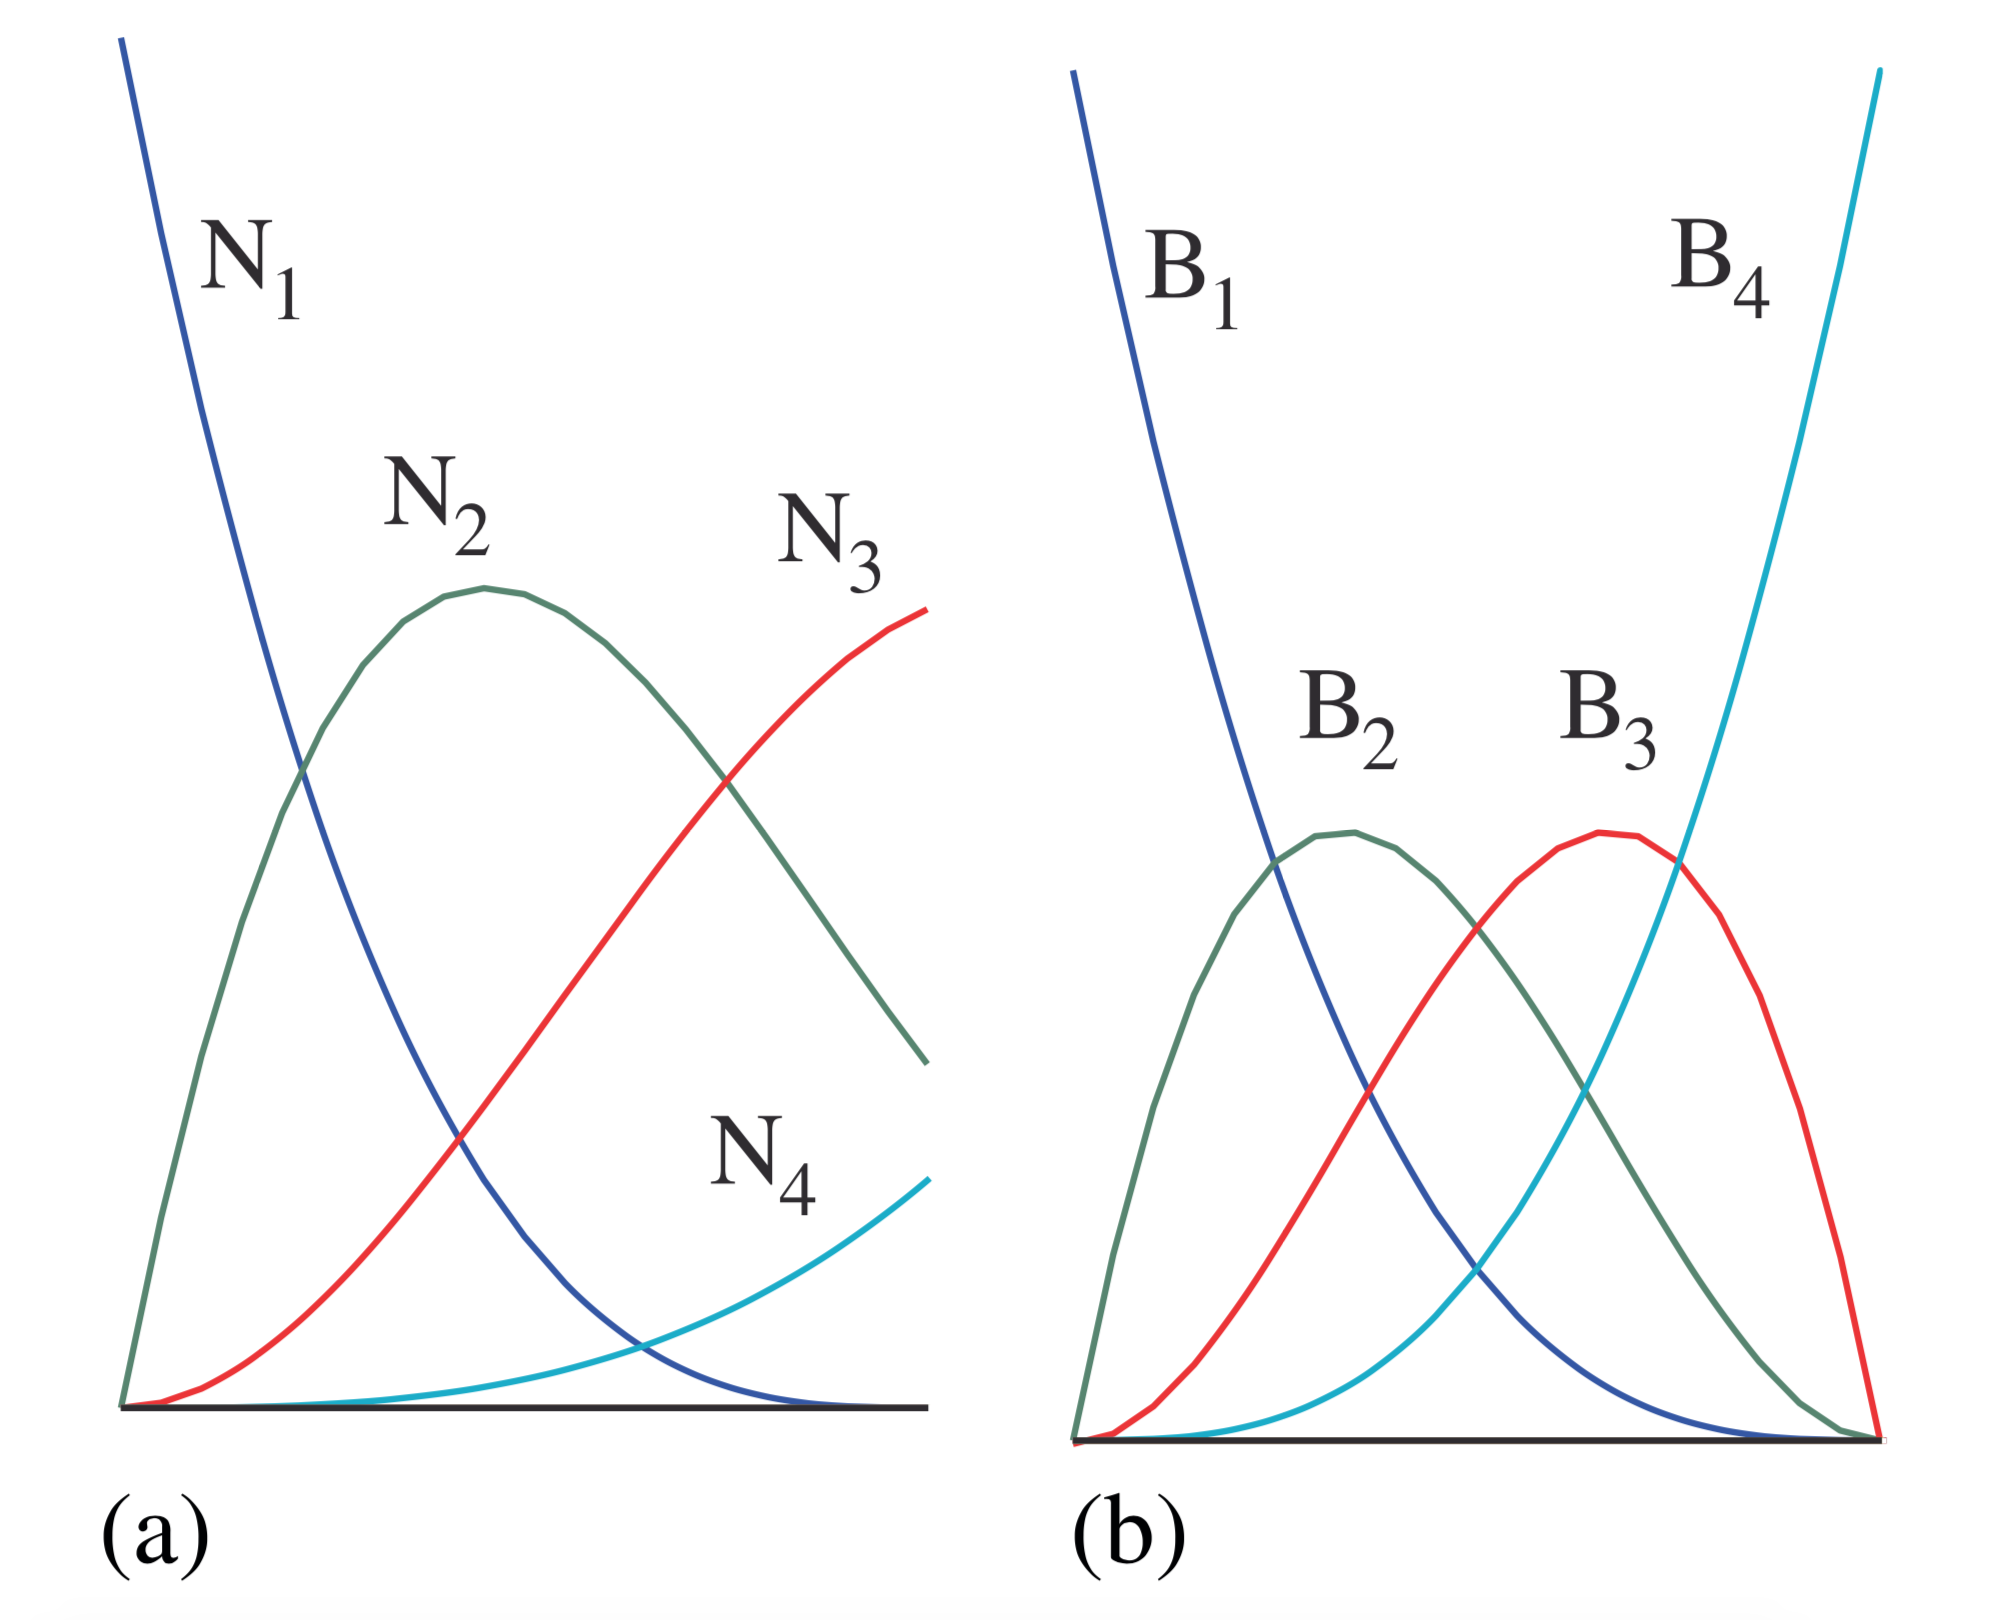
\includegraphics[width=4in]{./figures/Extracted_B-Spline}}
  \caption{\cite{borden_isogeometric_2011} B-Spline bases over a knot span (as in (a), $[0,1]$) can be written as linear combination of Bernstein bases (b) over their unit domain. The extraction operator stores the coefficients of these linear combinations.}
  \label{fig:extracted}
\end{figure}

\end{document}